\chapter{Specifica dei Requisiti}
Per avere una visione chiara di ciò che si deve costruire, quindi una descrizione dettagliata dei requisiti, sono stati effettuati dei colloqui con degli stakeholders e delle sessioni di "brainstorming" tra i componenti del gruppo. In seguito si è costruito un diagramma dei casi d'uso i quali sono stati poi descritti dettagliatamente.
\\Prima di elencare e descrivere i casi d'uso, è necessario identificare gli attori che caratterizzeranno il sistema.

\section{Attori Primari}
\begin{figure}[H]
	\centering
	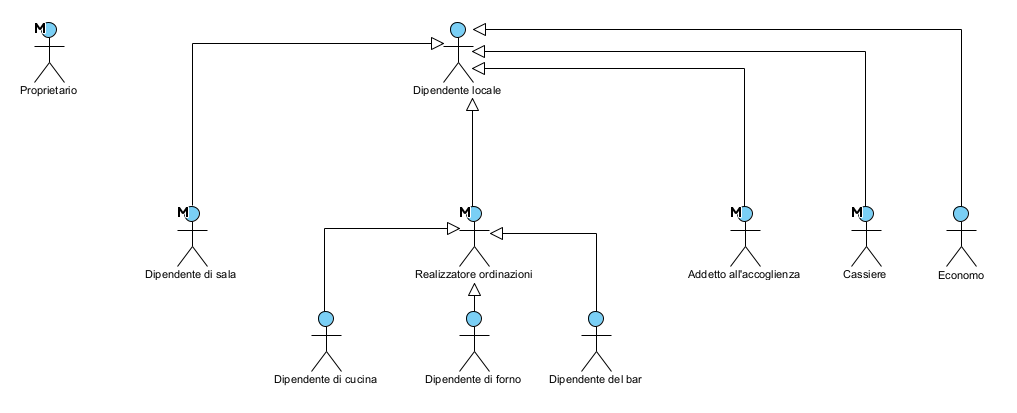
\includegraphics[width=\textwidth]{Immagini/AttoriPrimari.png}
\end{figure}

\begin{itemize}
	\item Dipendente di sala: deve interagire con il cliente e prendere le ordinazioni in maniera tale che vengano smistate, tramite il sistema alle varie attività del locale;
	\item Dipendenti di cucina/forno/bar: usano il sistema per ricevere i vari ordini e per notificare un completamento di essi;
	\item Addetto all'accoglienza: usa il sistema per visualizzare i tavoli disponibili ed assegnarli ai clienti;
	\item Cassiere: richiede al sistema il conto totale di un cliente interessato per completare il pagamento;
	\item Economo: si occupa della gestione delle merci ovvero l'aggiornamento delle quantità presenti in magazzino (in base alle vendite effettuate dalla sala e dalle richieste dei realizzatori di ordinazioni);
	\item Proprietario: può usare il sistema per aggiungere e rimuovere dipendenti, consultare dati come vendite, guadagni, quantità di merci.
\end{itemize}
Nella realtà non tutti gli attori descritti corrisponderanno a persone fisiche differenti, infatti alcuni dipendenti potranno assumere le funzionalità di più attori (ad esempio un dipendente di sala potrebbe ricoprire anche il ruolo di addetto all'accoglienza). A tal proposito quindi si è scelto di intendere gli attori come \textbf{ruoli} che un dipendente reale possa ricoprire.

\section{Attori Finali}
\begin{figure}[H]
	\centering
	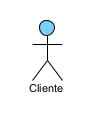
\includegraphics[width=0.12\textwidth]{Immagini/AttoriFinali.png}
\end{figure}

\begin{itemize}
	\item Cliente: pur non interagendo con il sistema, è direttamente interessato in alcuni suoi casi d'uso in quanto gli consentono di usufruire del servizio del locale
\end{itemize}
\newpage

\section{Tabella Attori-Obiettivi}
Dopo aver identificato a pieno gli attori che utilizzeranno il sistema, bisogna associare ad ogni attore i suoi obiettivi.
\begin{table}[!h]
	\centering
	\begin{tabular}{|p{0.3\linewidth}|p{0.65\linewidth}|}
		\hline
		\rowcolor{Red}
		Attore & Obiettivi \\
		\hline
		\hline
		\multirow{9}{6em} {Proprietario} & Inserimento di un dipendente \\
		& Rimozione di un dipendente \\ & Modifica dei ruolo di un dipendente \\
		& Visualizzazione dei dipendenti \\
		& Inserimento di un tavolo\\
		& Rimozione di un tavolo\\
		& Modifica di un tavolo\\
		& Visualizzazione dei tavoli \\
		& Inserimento di prodotti nel menu \\
		& Rimozioni di prodotti dal menu \\
		& Modifica di prodotti del menu \\
		& Visualizzazione del menu completo \\
		
		\hline
		\multirow{4}{6em} {Dipendente di sala} 
		& Creazione di un'ordinazione per un cliente  \\
		& Rimozione di un'ordinazione \\ 
		& Modifica di un'ordinazione \\
		& Visualizzazione delle ordinazioni \\
		\hline
	
		\multirow{3}{6em} {Accoglienza} 
		& Assegnazione di un tavolo a dei clienti  \\
		& Modifica dello stato di un tavolo (libero, occupato, riservato, ecc.) \\ 
		& Visualizzazione di tutti i tavoli \\
		\hline	
		
		\multirow{1}{6em} {Cassiere} 
		& Generazione vendita di un tavolo (pagamento dei clienti)\\ 
		\hline
		
		\multirow{2}{7em} {Realizzatore di ordinazione} 
		& Visualizzazione degli ordini per area (cucina, bar, forno)  \\
		& Notifica completamento ordinazione \\ 
		\hline
		
		\multirow{4}{6em} {Economo} 
		& Inserimento di una merce  \\
		& Modifica di una merce \\ 
		& Rimozione di una merce \\
		& Visualizzazione di una merce \\
		\hline
	\end{tabular}
\end{table}
\\Gran parte degli obiettivi riguardano operazioni \textit{CRUD} (Create, Read, Update, Delete) che possono essere raggruppate in un solo obiettivo.

\newpage
\section{Diagramma dei Casi D'Uso}
Tutti gli obbiettivi CRUD dei vari attori sono stati inglobati in un unico caso d'uso con il prefisso \textbf{Gestisci}, per indicare le operazioni che racchiudono.
\\
\\
\begin{centering}  
	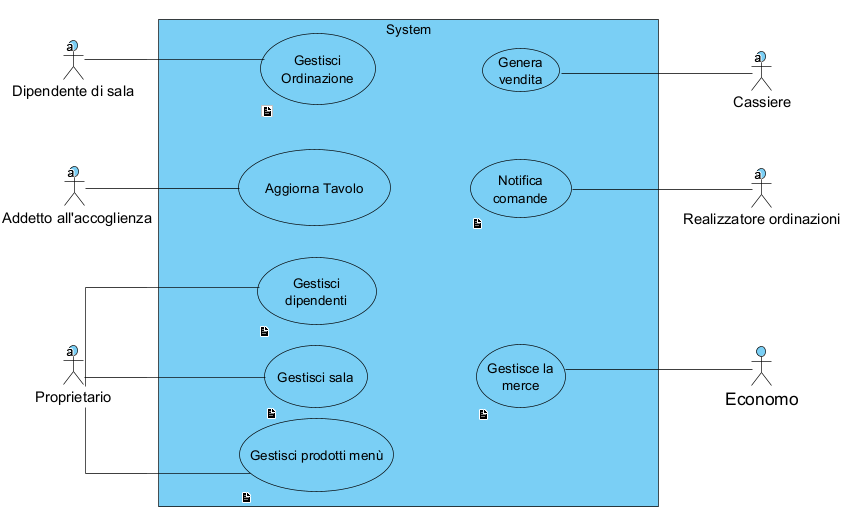
\includegraphics[width=\textwidth]{Immagini/DiagrammaCasiUso.png}
\end{centering}

\subsection{Descrizione Breve}
\subsubsection{Gestisci Ordinazione}
Come descritto in precedenza questo caso d'uso racchiude le operazioni CRUD riguardo ad un'ordinazione di uno o più clienti. Il cameriere infatti deve essere in grado di creare un'ordinazione per un cliente e poterla in seguito modificare, visualizzare o addirittura rimuovere dal sistema.

\subsubsection{Aggiorna Tavolo}
L'addetto all'accoglienza si occupa di far accomodare i clienti nella sala. Il suo obiettivo è quindi avere una visione completa dei tavoli comunicando tramite il sistema  quali tavoli hanno clienti in attesa di ordinazione, quali sono liberi e quali sono occupati.

\subsubsection{Gestisci Dipendenti}
Il proprietario può aggiungere/rimuovere dipendenti dal sistema ed inoltre è in grado di decidere/modificare i ruoli o il ruolo di ogni dipendente durante il servizio.

\subsubsection{Gestisci Sala}
Il proprietario può indicare l'identificativo di ogni tavolo in relazione alla sala in cui appartiene. Gli altri dipendenti quindi posso accedere tramite l'identificativo a tutte le informazioni che riguardano i tavoli (numero di persone accomodate, lista dei prodotti ordinati, ecc).

\subsubsection{Gestisci Prodotti Menù}
Il proprietario può effettuare operazioni CRUD per la gestione del menù del locale.

\subsubsection{Genera Vendita}
Il compito del cassiere è quello di registrare il pagamento dei clienti in relazione a ciò che hanno ordinato. Esso quindi deve poter risalire tramite il tavolo a tutti gli ordini associati ai clienti per ricavare il prezzo complessivo da pagare.

\subsubsection{Notifica Ordinazione}
Per rendere il sistema quanto più automatizzato possibile, i realizzatori di ordinazioni (cuoco, pizzaiolo, etc.) devono notificare il completamento di un'ordinazione tramite il sistema. In questo modo, inviando una notifica il sistema provvederà ad avvisare altri dipendenti in attesa di quel completamento.

\subsubsection{Gestisci Merce}
Ogni prodotto del menu è composto da un insieme di merci disponibili in magazzino. Il compito dell'economo è quindi quello di gestire le merci, per avere sotto controllo le merci in esaurimento. L'esaurimento di una merce comporta la non disponibilità di tutti i prodotti del menu che la contenevano.

\subsection{Descrizione Dettagliata}
La descrizione dettagliata è stata fatta solo per i casi d'uso di rilievo.

\begin{longtable}[htbp]{|p{0.3\linewidth}|p{0.65\linewidth}|}
	\hline
		\rowcolor{Blue}	
	\textbf{Titolo} & Gestisci Ordinazione \\[0.3cm]
	\hline
	\textbf{Livello} & Obiettivo Utente \\[0.3cm]
	\hline
	\textbf{Portata} & Applicazione Android o interfaccia Desktop \\[0.3cm]
	\hline
	\textbf{Attore Primario} & Dipendente di sala \\[0.3cm]
	\hline
	\multirow{8}*{\textbf{Parti Interessate}} 
	& \textendash \underline{Dipendenti di sala} (vogliono eseguire le loro mansioni) \\
	& \textendash \underline{Proprietario} (vuole che i clienti siano soddisfatti dal servizio) \\
	& \textendash \underline{Clienti} (vogliono essere serviti nel miglior modo possibile) \\
	& \textendash \underline{Realizzatore di ordinazioni} (vuole ricevere le ordinazioni) \\[0.3cm]
	\hline
	\multirow{8}*{\textbf{Pre-Condizioni}}
	& \textendash Il dipendente di sala non può gestire ordinazioni dei tavoli non suoi \\
	& \textendash Il dipendente di sala non può aggiungere prodotti ad ordinazioni già completate \\
	& \textendash Il dipendente di sala non può rimuove prodotti in lavorazione di una ordinazione \\
	& \textendash Il dipendente di sala non può rimuovere merce ad un prodotto in lavorazione \\[0.3cm]
	\hline
	\multirow{5}*{\textbf{Garanzia di successo}}
	& \textendash Una ordinazione viene creata/modificata/rimossa \\
	& \textendash Una notifica viene inviata ad un realizzatore di ordinazione \\
	& \textendash La merce numerabile costituente i prodotti viene riservata per l’ordinazione \\[0.3cm]
	\hline
	\multirow{5}*{\textbf{Scenario Principale}} 
	& 1. Dipendente di sala visualizza i tavoli in attesa di ordinazione di una sala \\
	& 2. Dipendente di sala seleziona un tavolo \\\
	& 3. Dipendente di sala visualizza ordinazioni tavolo \\
	& 4. Dipendente di sala visualizza ordinazione\\[0.3cm]
	\hline
	\newpage
	\multirow{28}*{\textbf{Estensioni}}
	& 3.A Dipendente di sala inizia ordinazione a tavolo \\
	& 4.A Cliente comunica i prodotti \\
	& 5.A Il dipendente di sala inserisce prodotti con eventuali merci aggiuntive \\
	& 6.A Il cliente comunica preferenza di consegna per prodotti \\
	& 7.A Il dipendente di sala inserisce la preferenza di consegna \\
	& 8.A Il dipendente di sala aggiunge ordinazione \\
	& 9.A Il sistema viene aggiornato \\
	& 10.A Vengono inviate notifiche in maniera  intelligente ai realizzatori di ordinazioni \\
	& \\
	& 3.B Il dipendente di sala rimuove una ordinazione \\
	& 4.B Il sistema viene aggiornato \\
	& 5.B Viene notificato l’evento ad eventuali realizzatori precedentemente notificati \\
	& \\
	& 4.C Cliente comunica al dipendente di modificare un prodotto all'interno di un'ordinazione \\
	& 5.C Dipendente di sala modifica l'ordinazione con i nuovi prodotti \\
	& 6.C Dipendente di sala inoltra la modifica \\
	& 7.C Il sistema inoltra la modifica ai corrispondenti realizzatori \\
	
	& \\
	& 4.D Cliente comunica al dipendente di aggiungere un prodotto all'interno di un'ordinazione \\
	& 5.D Dipendente aggiunge il prodotto (o i prodotti) all'ordinazione \\
	& 6.D Il sistema viene aggiornato e invia una notifica ai realizzatori \\
	
	& \\
	& 4.E Cliente comunica al dipendente di rimuovere un prodotto all'interno di un'ordinazione \\
	& 5.E Dipendente rimuove il prodotto (o i prodotti) all'ordinazione \\
	& 6.E Il sistema viene aggiornato e invia una notifica ai realizzatori \\[0.3cm]
	
	\hline
	\multirow{10}*{\textbf{Scenari Alternativi}}
	& 4.A.1 Prodotto comunicato non è disponibile \\
	& 4.A.2 Ripeti 4.A \\
	& \\
	& 3.B.1 Ordinazione non rimovibile (già completata) \\
	& 3.B.2 Ripeti 3.B \\
	& 4.C.1 L'ordinazione non è modificabile (poichè in lavorazione) \\
	& 4.C.2 Ripeti 4.C \\
	& \\
	& 4.D.1 Il prodotto non è disponibile \\
	& 4.D.2 Ripeti 4.D \\
	& \\
	& 4.E.1 Il prodotto non è rimovibile (poichè in lavorazione) \\
	& 4.E.2 Ripeti 4.E \\[0.3cm]
	\hline
\end{longtable}
\vfill
\begin{longtable}[htbp]{|p{0.3\linewidth}|p{0.65\linewidth}|}
	\hline
	\rowcolor{Green}
	\textbf{Titolo} & Notifica Ordinazione \\[0.3cm]
	\hline
	\textbf{Livello} & Obiettivo Utente \\[0.3cm]
	\hline
	\textbf{Portata} & Applicazione Android o interfaccia Desktop \\[0.3cm]
	\hline
	\textbf{Attore Primario} & Realizzatore di ordinazione \\[0.3cm]
	\hline
	\multirow{8}*{\textbf{Parti Interessate}} 
	& \textendash \underline{Realizzatore di ordinazione} (vuole notificare l’aver completato uno o più lavori, altri realizzatori inoltre possono aspettare questa notifica come segnale per poter iniziare il loro lavoro). \\
	& \textendash \underline{Cliente} (vuole ricevere l’ordinazione). \\
	& \textendash \underline{Proprietario} (vuole che cliente riceva l’ordinazione) \\[0.3cm]
	\hline
	\multirow{1}*{\textbf{Pre-Condizioni}}
	& \textendash L'ordinazione da notificare esiste \\[0.3cm]
	\hline
	\newpage
	\multirow{6}*{\textbf{Garanzia di successo}}
	& \textendash Prodotto in ordinazione viene posto in stato di terminato \\
	& \textendash Qualora i prodotti di tutta l’ordinazione vengano posti come terminati allora anche l’ordinazione stessa viene posta come terminata \\[0.3cm]
	\hline
	\multirow{7}*{\textbf{Scenario Principale}} 
	& 1. Realizzatore richiede ordinazioni al sistema \\
	& 2. Il sistema restituisce le ordinazioni che può eseguire \\
	& 3 Il realizzatore seleziona un prodotto \\
	& 4 Il sistema restituisce i dati del prodotto \\
	& 5. Il realizzatore notifica il completamento del prodotto \\
	& 6. Il sistema si aggiorna \\
	& 7. Il sistema sblocca prodotti pendenti \\[0.3cm]
	\hline
	
	\multirow{5}*{\textbf{Estensioni}}
	& 5.A Il prodotto completato era l'ultimo \\
	& 6.A Il sistema aggiorna lo stato dell'ordinazione \\
	& 7.A Il sistema invia un'ordinazione pendente per altri realizzatori di ordinazione in attesa di quel completamento	\\[0.3cm]
	\hline
	\multirow{1}*{\textbf{Scenari Alternativi}}
	& 7.B.1 Non ci sono ordini pendenti \\[0.3cm]
	\hline
\end{longtable}
\newpage
\section{Requisiti non funzionali}
Il sistema oltre a realizzare i requisiti descritti precedentemente deve rispettare dei vincoli di funzionamento. Tutti i requisiti non funzionali vengono descritti tramite delle specifiche supplementari di tipo \textbf{FURPS+}

\subsection{Funzionalità}
Per tutti i casi d'uso deve esistere una gestione degli errori ottimale. Durante il funzionamento dell'applicazione, il sistema non deve interrompersi a causa degli errori non gestiti.

\subsection{Utilizzabilità}
L'interfaccia utente deve essere semplice e intuitiva. Il software è pensato per garantire un'esperienza migliore per il cliente che usufruisce del servizio; il dipendente deve poter interagire con il sistema nel modo più veloce possibile.
\\Inoltre l'applicativo è pensato per essere installato in modo "mobile" su un qualsiasi smartphone, per ridurre al minimo i costi per dispositivi dedicati.

\subsection{Affidabilità}



\subsection{Prestazioni}
Il sistema deve funzionare in Real-Time. La gestione delle ordinazioni, soprattutto, deve poter rispondere immediatamente alle variazioni, modifiche e aggiunta di eventuali ordinazioni nel sistema, per notificare velocemente coloro che dovranno realizzarle.

\subsection{Sostenibilità}
Nel lato "mobile" il sistema deve adattarsi alla maggior parte degli smartphone in commercio, onde evitare problemi di compatibilità. \\
Nel lato "desktop" il sistema deve essere portabile per poter essere configurato in un qualunque ambiente. 
